\documentclass[8pt]{article}
\usepackage{graphicx}
	\setkeys{Gin}{width=0.4\textwidth}
\usepackage[a4paper]{geometry}
\usepackage{listings}
\newcommand*{\deriv}{\ensuremath{\mathrm{d}}}
\twocolumn
\begin{document}
	\author{Jonathan Cancio \\ Oliver Atienza \\ Justin Balderas \\ 
	Reyster Fresco \\ Yna Ojeda \\ Ethan Tan \\ Marc Teves \\ Troy Valdez}
	\title{CS 131 MP2: Analysis of stock market prices as a function of previous price, volume, and momentum}
	\maketitle
	\section{Abstract}
	% Make sure to always have one sentence per line.
	Stock prices seem to be unpredictable.
	Predicting the future price of shares in a particular company will allow stock traders to make more profitable trading strategies.
	The group tried to predict the closing price of seven different companies on 24 May 2018. 
	The group performed a linear regression on their closing price, trading volume, and closing price momentum over varying timespans.
	The prediction error was found to be (to be continued...)
	\section{Introduction}

	Stock prices are unpredictable because there are simply too many factors that can influence the price of shares.
	While it would not be impossible to gather all the possible factors that could affect the price of a specific stock and make a mathematical equation describing how each factors into predicting the future price of a stock, it is likely that there are too many factors for any human built system to track.

	The most obvious way of making money in the stock market via trading stocks is \textit{arbitrage}, more commonly known as "buy low, sell high".
	Less known is the more effective technique called \textit{momentum investing}, summarized as "buy high, sell higher". 

	Momentum investing became a popular strategy after investors and economists noticed that if a stock has been performing well over a time period of three to twelve months, then it will continue to do well.
	That is, if the price of a stock has had high returns for a long time, then it will continue to have high returns.
	On the other hand, if a stock has had poor returns for a long time, then it will continue to have low returns.

	This tendency to stay increasing or decreasing is known as \textit{momentum}, and can be quantified as the derivative of stock price at a specific point in time.

	$$ m_{t} = \frac{\deriv P(t)}{\deriv t} $$

	where $P(t)$ is the price at time $t$.

	If momentum investing is a good strategy, then there is some function

	$$ P(t, m) $$

	that reasonably predicts $P(t)$ at some future $t$. If $$P(t,m)$$ was a 
	linear sum 

	$$ P(t,m) = \alpha f(t) + \beta m_{t} $$

	then it must be that $\beta > 0$, which indicates that the momentum 
	positively influences stock prices, making the equation consistent with 
	momentum investing theory.

	A good guess for $P(t,m)$, the \textit{predictor} would be 

	$$ P(t_{k+1},m) = \alpha P(t_{k}) + \beta V(t_{k}) + \gamma m_{t_k}$$

	This equation simply says that the current price is a linear sum of the previous price, the previous trading volume, and the momentum.

	In the real world, instead of a function $P(t)$, instead there are several data points that give the price $P$ for each point in time $t$.
	Thus, its derivative, the value for $m_{t}$, cannot be solved analytically, but it can be solved numerically.
	Instead of finding the exact value of the derivative, it is estimated.

	One way to estimate the derivative of a function is the \textit{centered difference formula}

	$$ m_{t} = \frac{\deriv P(t)}{\deriv t} = \frac{P(t+h) - P(t-h)}{2h} $$

	This equation uses two data points before and after the point of interest to obtain an approximation of $m_{t}$.

	With this equation, it is now possible to obtain the momentum without knowledge of $P(t)$, as long as $P(t+h)$ and $P(t-h)$ are known.

	On account of the inaccuracy incurred by solving for the derivative analytically, the predictor is modified:

	$$ P(t_{k+1},m) = \alpha P(t_{k}) + \beta V(t_{k}) +
	\gamma m^{h=22}_{t_k} + \sigma m^{h=7}_{t_k}$$

	Now the predictor uses two momentums computed over different time intervals.
	Finding the value for these coefficients is as simple as applying linear least squares regression over a set of data points.

	The group will find the optimal coefficients for seven companies in the Philippine stock exchange:
	\begin{itemize}
		\item AP
		\item CEB
		\item CHIB
		\item GTCAP
		\item MBT
		\item MEG
		\item RLC
	\end{itemize}

	\section{Methodology}

	A dataset of the Philippine stock exchange was retrieved from Kaggle.
	The seven companies were chosen because of their relative volatility and their influence to the stock market as a whole.

	\begin{figure}[h]
		\centering
		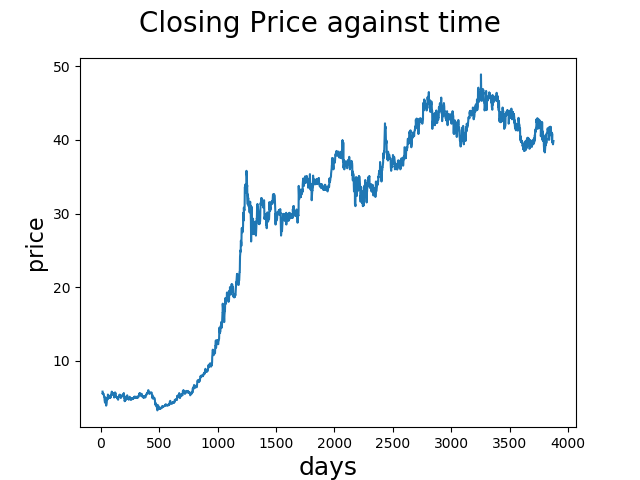
\includegraphics{ap_closing_price.png}
		\caption{Closing price graph of GTCAP, showing its volatility}
		\label{fig:gtcap_graph}
	\end{figure}

	\subsection{Preprocessing}
		\subsubsection{Removing irrelevant companies}
		There were many companies in the dataset. The rows containing companies irrelevant to the study were removed.
		The remaining rows were grouped by company, then separated into seven \texttt{.csv} files.
		\subsubsection{Finding the right price}
		The dataset did not have data for all the points of interest.
		For example, during holy week, there were no entries because the stock market was closed.
		If the group needed an entry at time $t$, the entry at the greatest 
		$t_{prev}$ was considered, where $t_{prev} > t$
		\subsubsection{Extracting relevant features}
		Just as there were too many rows, there were some irrelevant columns in the dataset.
		The group only needed the company name, the closing price, the trading volume, and the date at which the trade occurred.
		Only those columns (features) were considered for the rest of the research.

	\subsection{Graphing}
	Four python scripts located in \texttt{python\_scripts/} were made to graph the four terms in the predictor over time.
	The module \texttt{matplotlib} was used to plot the resulting graphs.

	\subsection{Finding the right coefficients}
	The coefficients for the predictor for each of the companies were found using linear least squares regression.

	\section{Results and Discussion}

	\begin{figure}[h]
		\centering
		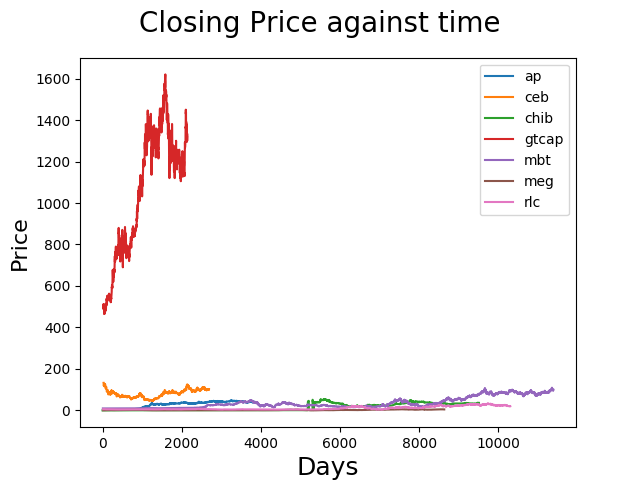
\includegraphics{all_closing_price.png}
		\caption{Graph of closing prices}
		\label{fig:close_price_graph}
	\end{figure}

	As shown in Figure~\ref{fig:close_price_graph}, most of the companies have an unpredictable looking price graph.

	\begin{figure}[h]
		\centering
		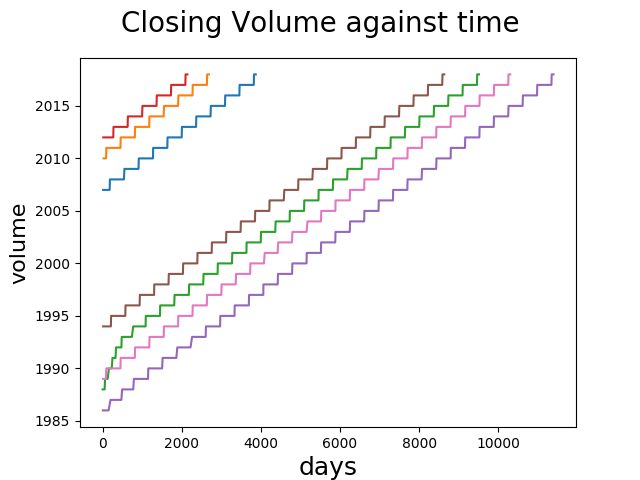
\includegraphics{all_closing_volume.png}
		\caption{Graph of closing volumes}
		\label{fig:close_volume_graph}
	\end{figure}

	In Figure~\ref{fig:close_volume_graph}, it shows the total volume of trades the company went over time.
	The graph exhibits a "stairs" pattern, showing the spikes in buying and selling when prices fluctuate.

	\begin{figure}[h]
		\centering
		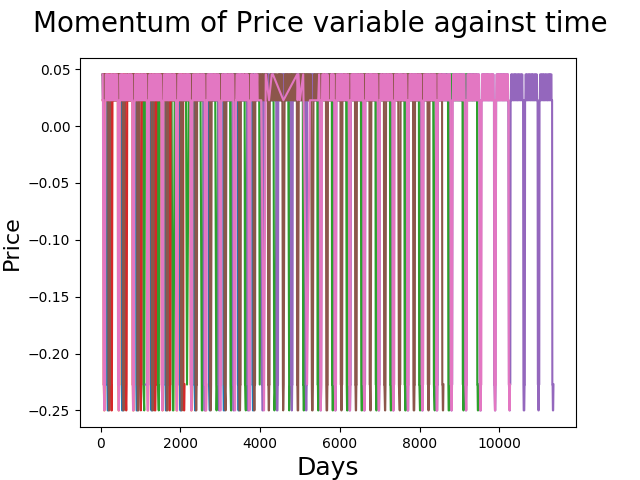
\includegraphics{all_momentum_step_22.png}
		\caption{Graph of closing price momentum with $h=22$}
		\label{fig:close_m22_graph}
	\end{figure}

	\begin{figure}[h]
		\centering
		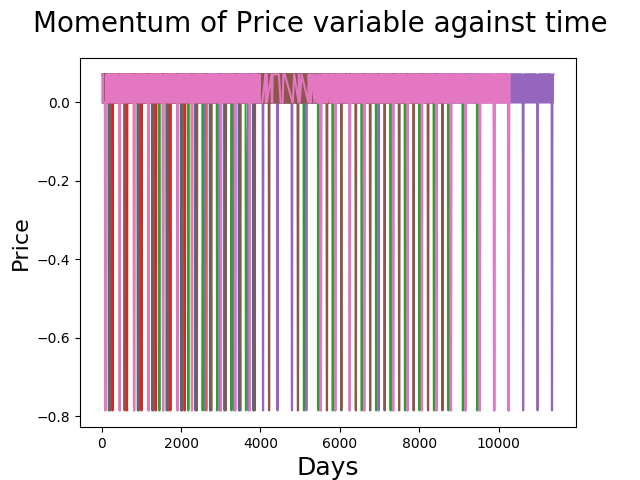
\includegraphics{all_momentum_step_7.png}
		\caption{Graph of closing price momentum with $h=72$}
		\label{fig:close_m7_graph}
	\end{figure}

	Stock prices tend to fluctuate the same way a heart beat wave fluctuates in an ECG monitor.
	The momentum graphs (shown in Figure~\ref{fig:close_m22_graph} and Figure~\ref{fig:close_m7_graph}), which is a derivative of the price graph, looks like a bunch of candle sticks.
	Each abrupt spike/drop in price gets converted into an impulse in the momentum that shoots upward/downward. 

	It is worth noting that the momentum reaches farther into the negative side than the positive side, for both graphs.
	The momentum graph for $h=22$ is less erratic and shows more stability, however the momentum graph for $h=7$ reflects the instantaneous derivative better.
	Going to a larger stepsize means trading off accuracy for stability.
	
	\begin{figure}[h]
		\begin{tabular}[h]{|c|c|c|c|c|}
			\hline
			Company & $\alpha$ & $\beta$ & $\sigma$ & $\gamma$ \\\hline
			AP & 0.999909308676 & 0.000000000893 & -0.002057696004 & 1.223340993478 \\\hline
			CEB & 1.223340993478 & 0.000000014819 & 0.040550002555 & 1.378957068841 \\\hline
			CHIB & 0.998817540958 & 0.000000000015 & 0.134914332815 & 1.571397313188\\\hline
			GTCAP & 0.999805323406 & 0.000000601056 & 0.430392355966 & 1.158406101105 \\\hline
			MBT & 0.999110807743 & 0.000000017390 & 0.089714560749 & 1.419385112693\\\hline
			MEG & 0.999526525917 & 0.000000000024 & -0.000000000024 & 1.501996489010 \\\hline
			RLC & 0.999311080033 & 0.000000003205 & 0.115358802114 & 1.392324898465 \\\hline
			Average & 0.999463266205 & 0.000000091058 & 0.110422779598 & 1.378286853826 \\\hline
		\end{tabular}
		\centering
		\caption{Table of computed optimal coefficient values}
	\end{figure}

	\section{Conclusion}
	\begin{thebibliography}{9}
		\bibitem{heath}
			Heath M.,

			\textit{Scientific Computing - An Introductory Survey}
	\end{thebibliography}
\end{document}
